\section{Introduction}
%% Chapter 3: functional diversity analyses
%Dormann 2012 Collinearity: a review of methods to deal with it and a simulation study evaluating their performance
% Mouillot et al 2014 
\section{Methods}
\subsection{Trait selection for functional diversity metric calculations}
In Chapter 1, I collected and imputed trait values for 10 traits across terrestrial vertebrates.
I randomly selected one trait dataset among the eight imputed datasets (see Chapter 1) for all subsequent analyses. Continuous traits were transformed to improve normality. A log-10 transformation was applied to all continuous traits except habitat breadth, which was square-rooted. Traits were centred and scaled to zero-mean and unit-variance.

All traits were considered for inclusion into the calculation of functional diversity metrics, except variables relating to species diet, as these were unavailable for reptiles. Deciding which traits to include in functional diversity metrics was a critical step, as the metrics can be sensitive to the number of traits included (Mouillot et al 2014). On the one hand, not including enough variables may lead to missing important areas in the multidimensional trait space. On the other hand, collinearity among the traits could create a form of redundancy in the trait space, biasing estimated functional metrics. As such, a pre-analysis clean-up of the data was necessary to select traits to include in the calculations.

To first assess if collinearity could be a problem, I used a clustering approach for mixed-type data (factor analysis of mixed type data, or FAMD, ref) to represent the contribution of each variables to principal components. The graph shows that body mass - longevity might e correlated and that BM-LCS could be negatively correlated.

\begin{figure}[h!]
\centering
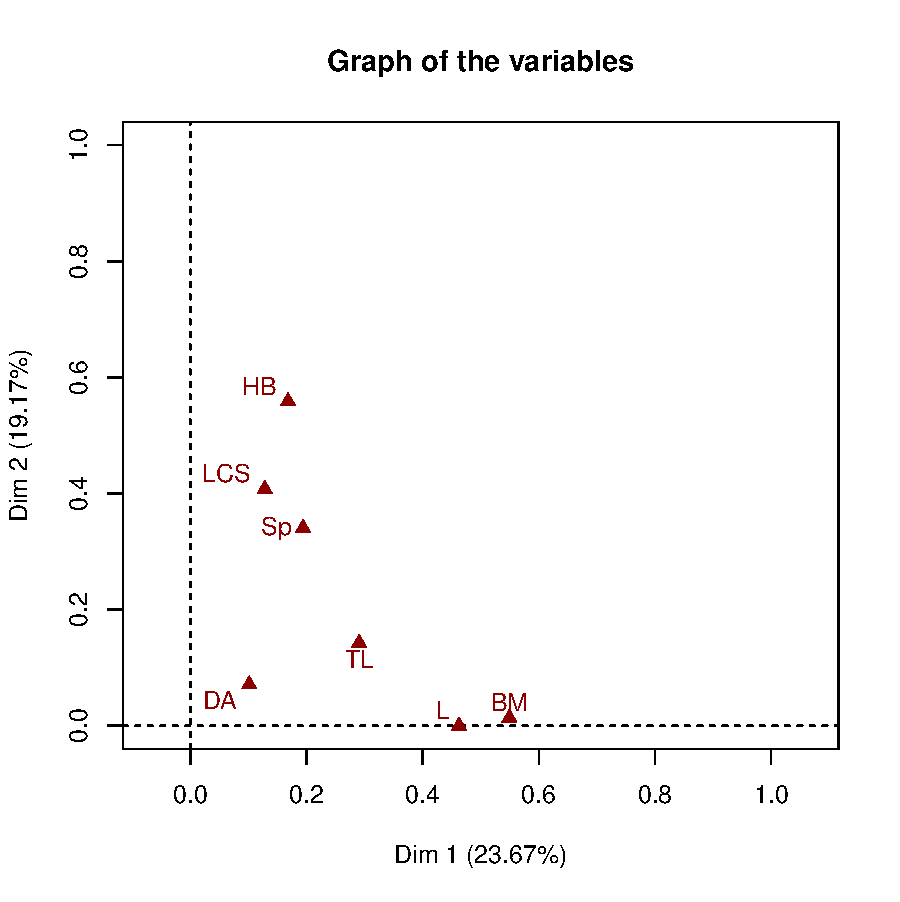
\includegraphics[scale=0.75]{figures/chapter3/Graph_traits_variables}
\caption[]{\textbf{}}
\label{}
\end{figure}

\begin{figure}[h!]
\centering
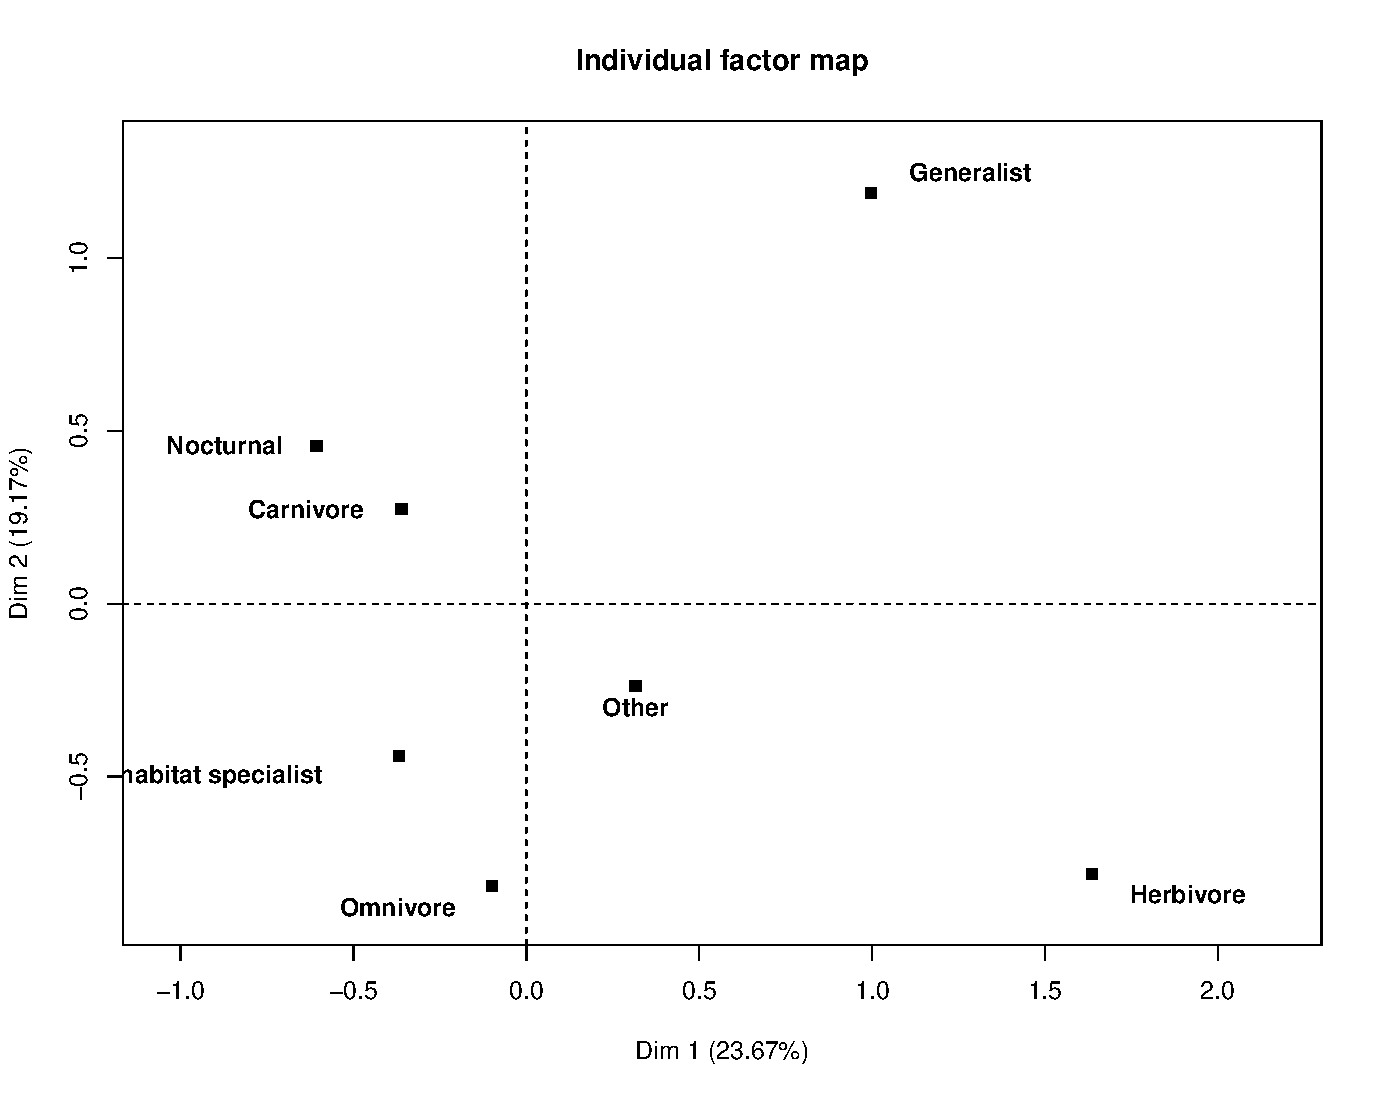
\includegraphics[scale=0.75]{figures/chapter3/Individual_factor_map}
\caption[]{\textbf{}}
\label{}
\end{figure}

\begin{figure}[h!]
\centering
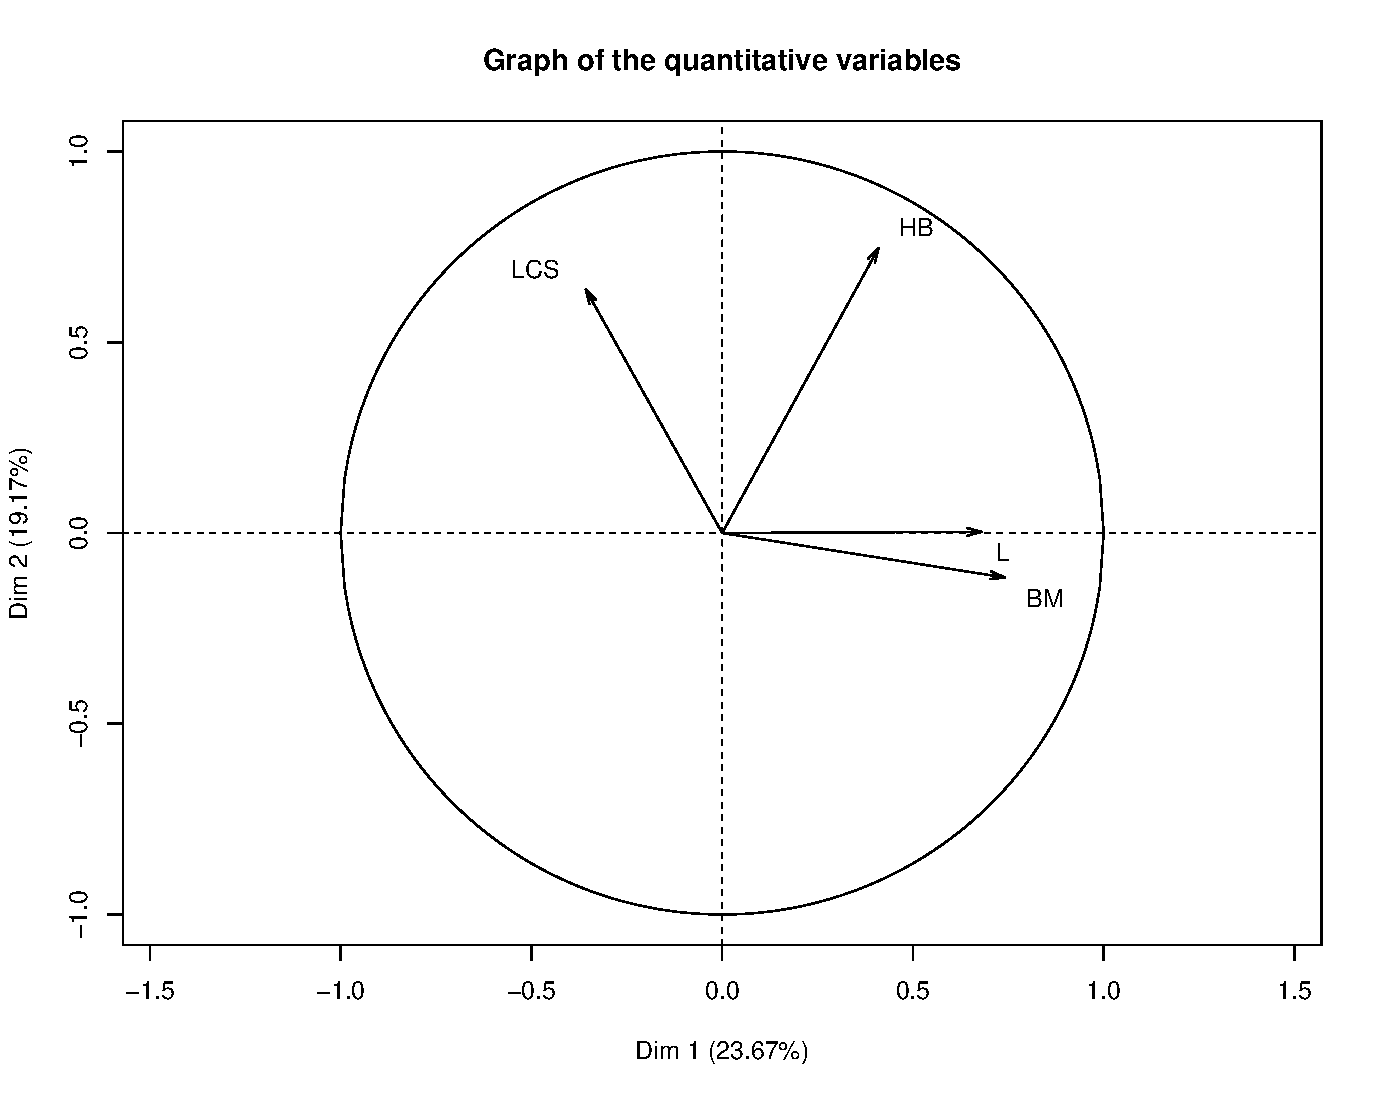
\includegraphics[scale=0.75]{figures/chapter3/Quantitative_variables}
\caption[]{\textbf{}}
\label{}
\end{figure}

Next, I assessed Pearson's pairwise correlation coefficients among continuous traits, as high correlations can be an indicator of collinearity. Body mass and longevity were the highest correlated variables (Table XX, correlation: 0.51), nevertheless below or close to the threshold usually used for detecting potential collinearity (threshold of 0.7, Dormann 2012). Moreover, the determinant of the correlation matrix was 0.67. Values close to 0 indicate high degrees of collinearity in the dataset, while values close to one indicate low degrees of collinearity. A stepwise selection process using variance inflation factors (VIF) also failed to detect multicollinearity among continuous traits (with a threshold of 5; all VIF$\leq$1.4).

Consequently, all candidate traits were selected for inclusion in the functional metrics calculation. The selected traits were: body mass; longevity; litter/clutch size; trophic level;  habitat breadth; degree of habitat specialisation; and diel activity.

\subsection{Calculation of functional diversity metrics across PREDICTS vertebrate communities}

\subsubsection{Dendrogram-based functional richness}
A Gower dissimilarity matrix was first computed from the trait dataset, using the gowdis R function (FD package). This distance matrix contained pairwise distances across all terrestrial vertebrates, based on their trait values. Gower distances allowed to include mixed type variables in the computation. In a second step, this dissimilarity matrix was clustered, to obtain a functional dendrogram, where species presenting similar functional characteristics were closer than more dissimilar species. I used the hclust function, which offers a range of clustering methods. As different clustering methods can have a strong influence on the output dendrogram, I selected the clustering method that best reflected the initial distances in the Gower matrix (correlation coefficient between cophenetic distances obtained from the cluster dendrograms and between the initial dissimilarities in the Gower matrix). The `average' method (unweighted pair group method with arithmetic mean, UPGMA) presented the best correlation coefficient and was as such selected. The resulting cluster dendrogram was a functional dendrogram with 34377 tips, where each tip represented a species. Species position in the tree depended on their functional attributes: species that were functionally more similar were more closely related in the tree.

Finally, functional richness was calculated across all PREDICTS sites. At each site, vertebrate community composition was assessed (species presence/absence), and the functional dendrogram was subsetted according to local community composition. For a site, functional richness was calculated as the sum of the branch length, from root to tip, for the local subset of the functional dendrogram (treedive).

% community matrices for each studies
194 studies to start with; presence absence matrices: 10 studies were excluded
for abundance matrices: 30 studies were excluded.

\subsection{Impact of land-use change on the functional diversity of vertebrate communities}

\section{Results}

\section{Discussion}
% sensitivity to trait inclusion
% traits that were not considered that could be important, noably home range, dispersal abilities, or volancy -- traits relating to species abilities to move.